%!TEX root=../../thesis_rui_almeida.tex
\section{Reconstruction Results}%
\label{sec:reconstruction_results}

Until now, this section was dedicated to explaining the theoretical and
computational aspects of the TomoSim software program.  In this section,
I will focus on the results that it produced, namely in what concerns
the tomographic reconstruction of an image based on the concentration of
selected atmospheric trace gases.

In TomoSim, a projection is the sum of the pixel lengths (the lengths of
the rays that traverse each pixel) for each ray and for the grid
mentioned in Section~\ref{sec:tomosim}. Unlike a real life situation,
the contents of the ROI are completely known and correspond to the
phantoms also described in Section~\ref{sec:tomosim} multiplied by a
given maximum number of molecules. Siddon's algorithm is used in this
process, and the final results of its application are the sinogram and
the system matrix. Figure~\ref{fig:sinograms} contains some examples of
these matrices, before and after the resorting operation described in
the last lines of
Section~\ref{sec:tomographic_algorithms_and_reconstruction_techniques}.

\begin{figure}[htpb]
    \centering
    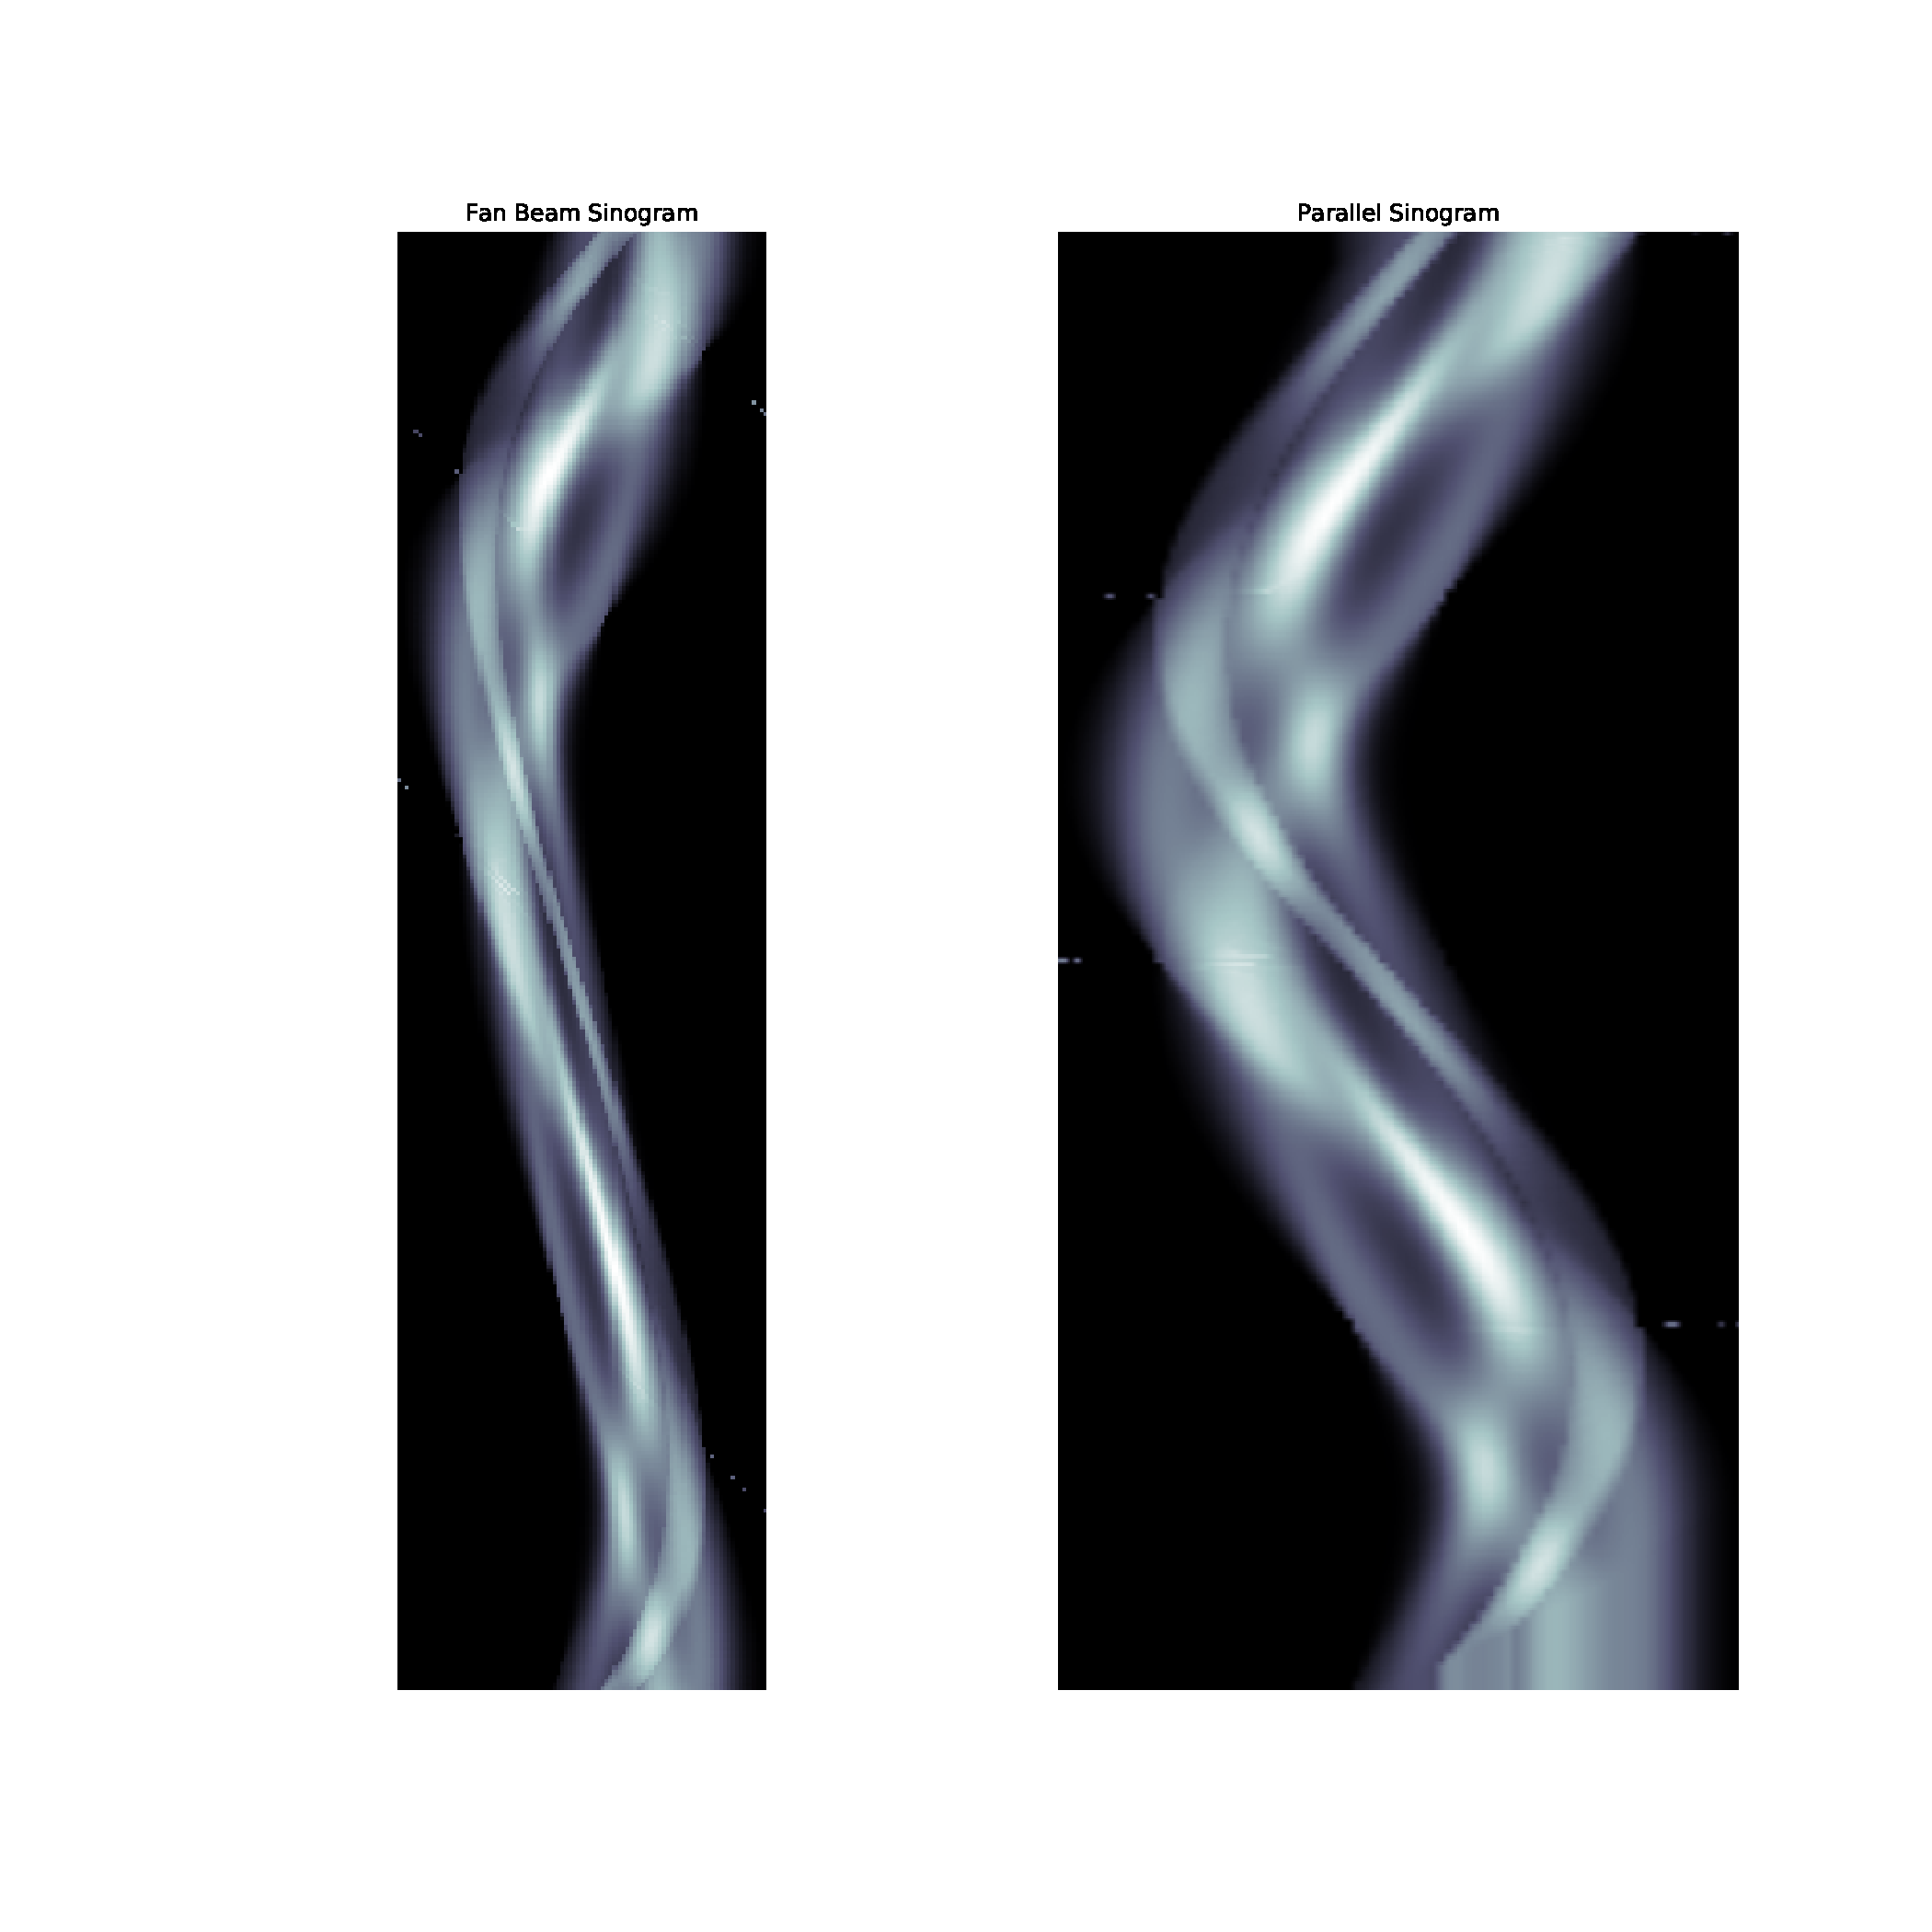
\includegraphics[clip, trim=7cm 4cm 3.2cm 3.5cm,
    width=.6\textwidth]{img/pdf/fanbeam_comparison.pdf}
    \caption{Sinogram examples: the new spectral phantom projection data
    at a projection interval of 1 degree. On the left, the projection
    data before resorting; on the right, the parallel projection data
    obtained after resorting the fan-beam line integrals.}
    \label{fig:sinograms}
\end{figure}

Images corresponding to the trace gas distribution within the ROI were
reconstructed using iterative and analytical methods. In
Figure~\ref{fig:rec_results}, one can see the reconstruction results for
the three tested methods when applied to the new spectral phantom;
Figure~\ref{fig:rec_errors} shows the graphical representation of the
reconstruction errors for the spectral phantom and is accompanied by
Table~\ref{tab:rec_errors}; and in Figure~\ref{fig:rec_comparison}, a
comparison between reconstructions with different $\Delta$ values is
presented, also for the new spectral phantom. 

\begin{figure*}[t]
    \centering
    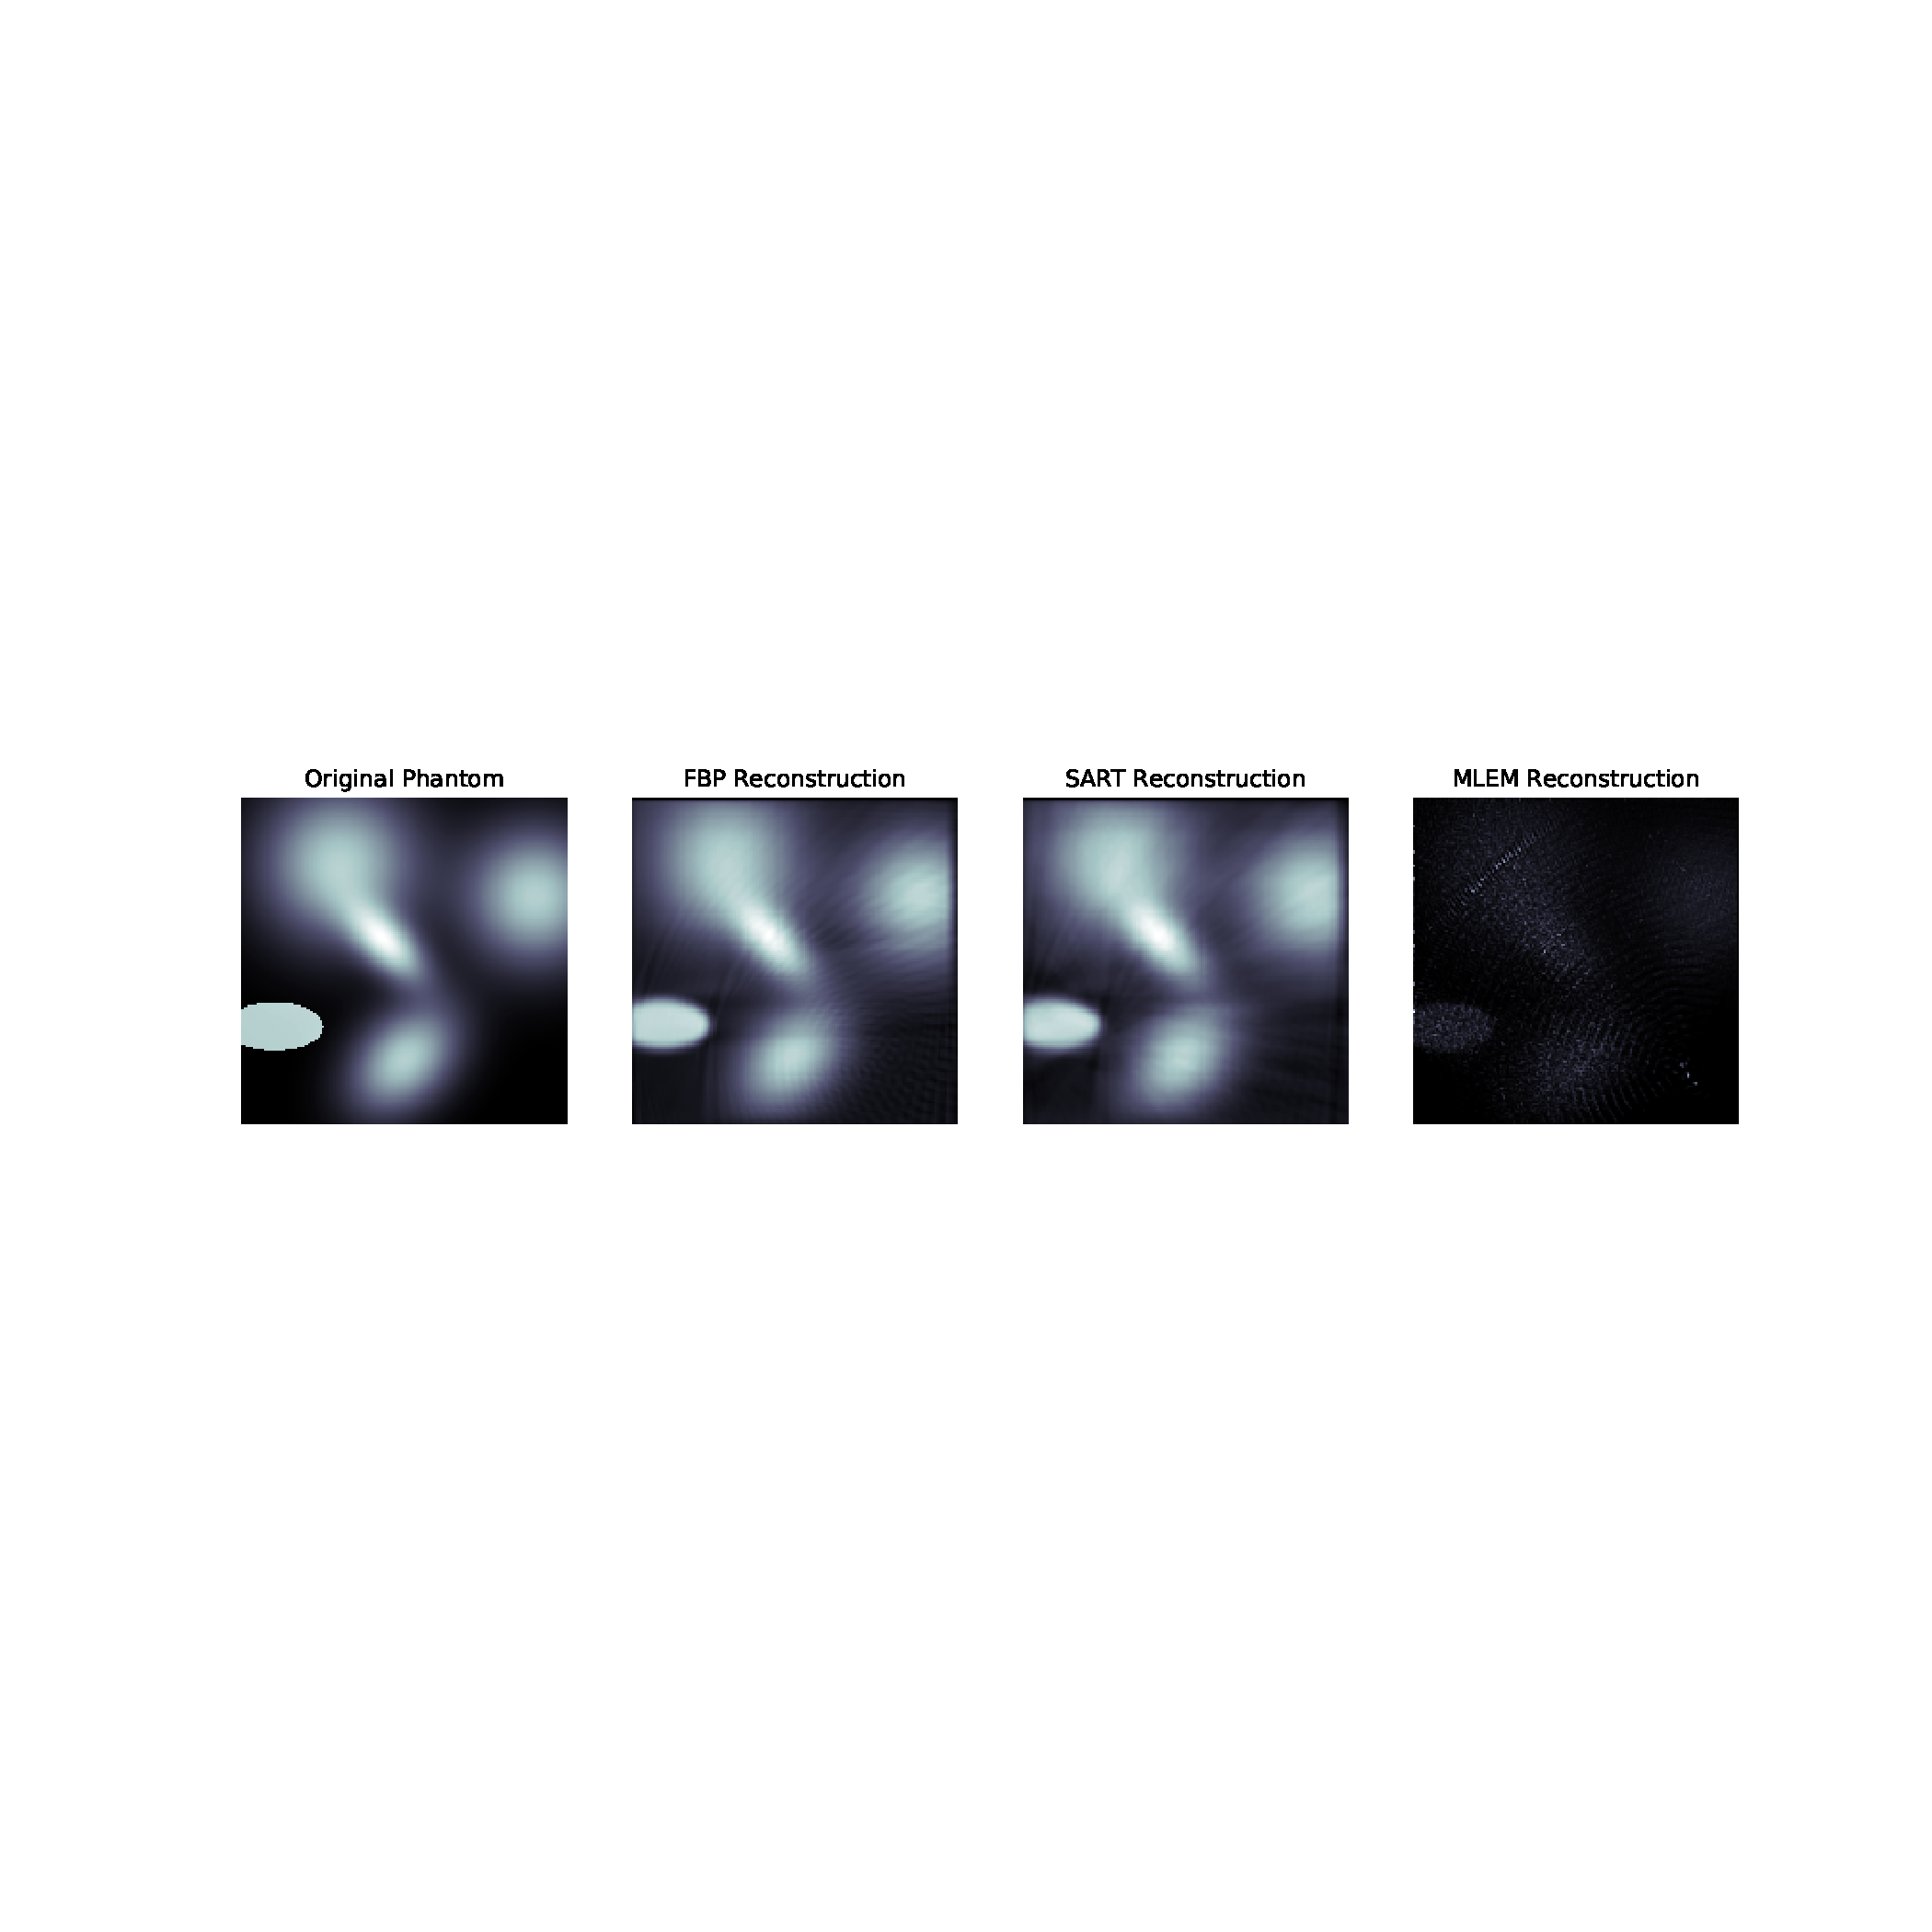
\includegraphics[clip, trim=4cm 15cm 3cm 14cm,
    width=\textwidth]{img/pdf/rec_compilation_1.pdf}
    \caption{Tomographic reconstruction results, projection interval of
    1 degree. From left to right: original phantom, FBP reconstruction,
    SART reconstruction, MLEM reconstruction}
    \label{fig:rec_results}
\end{figure*}

\begin{figure*}[t]
    \centering
    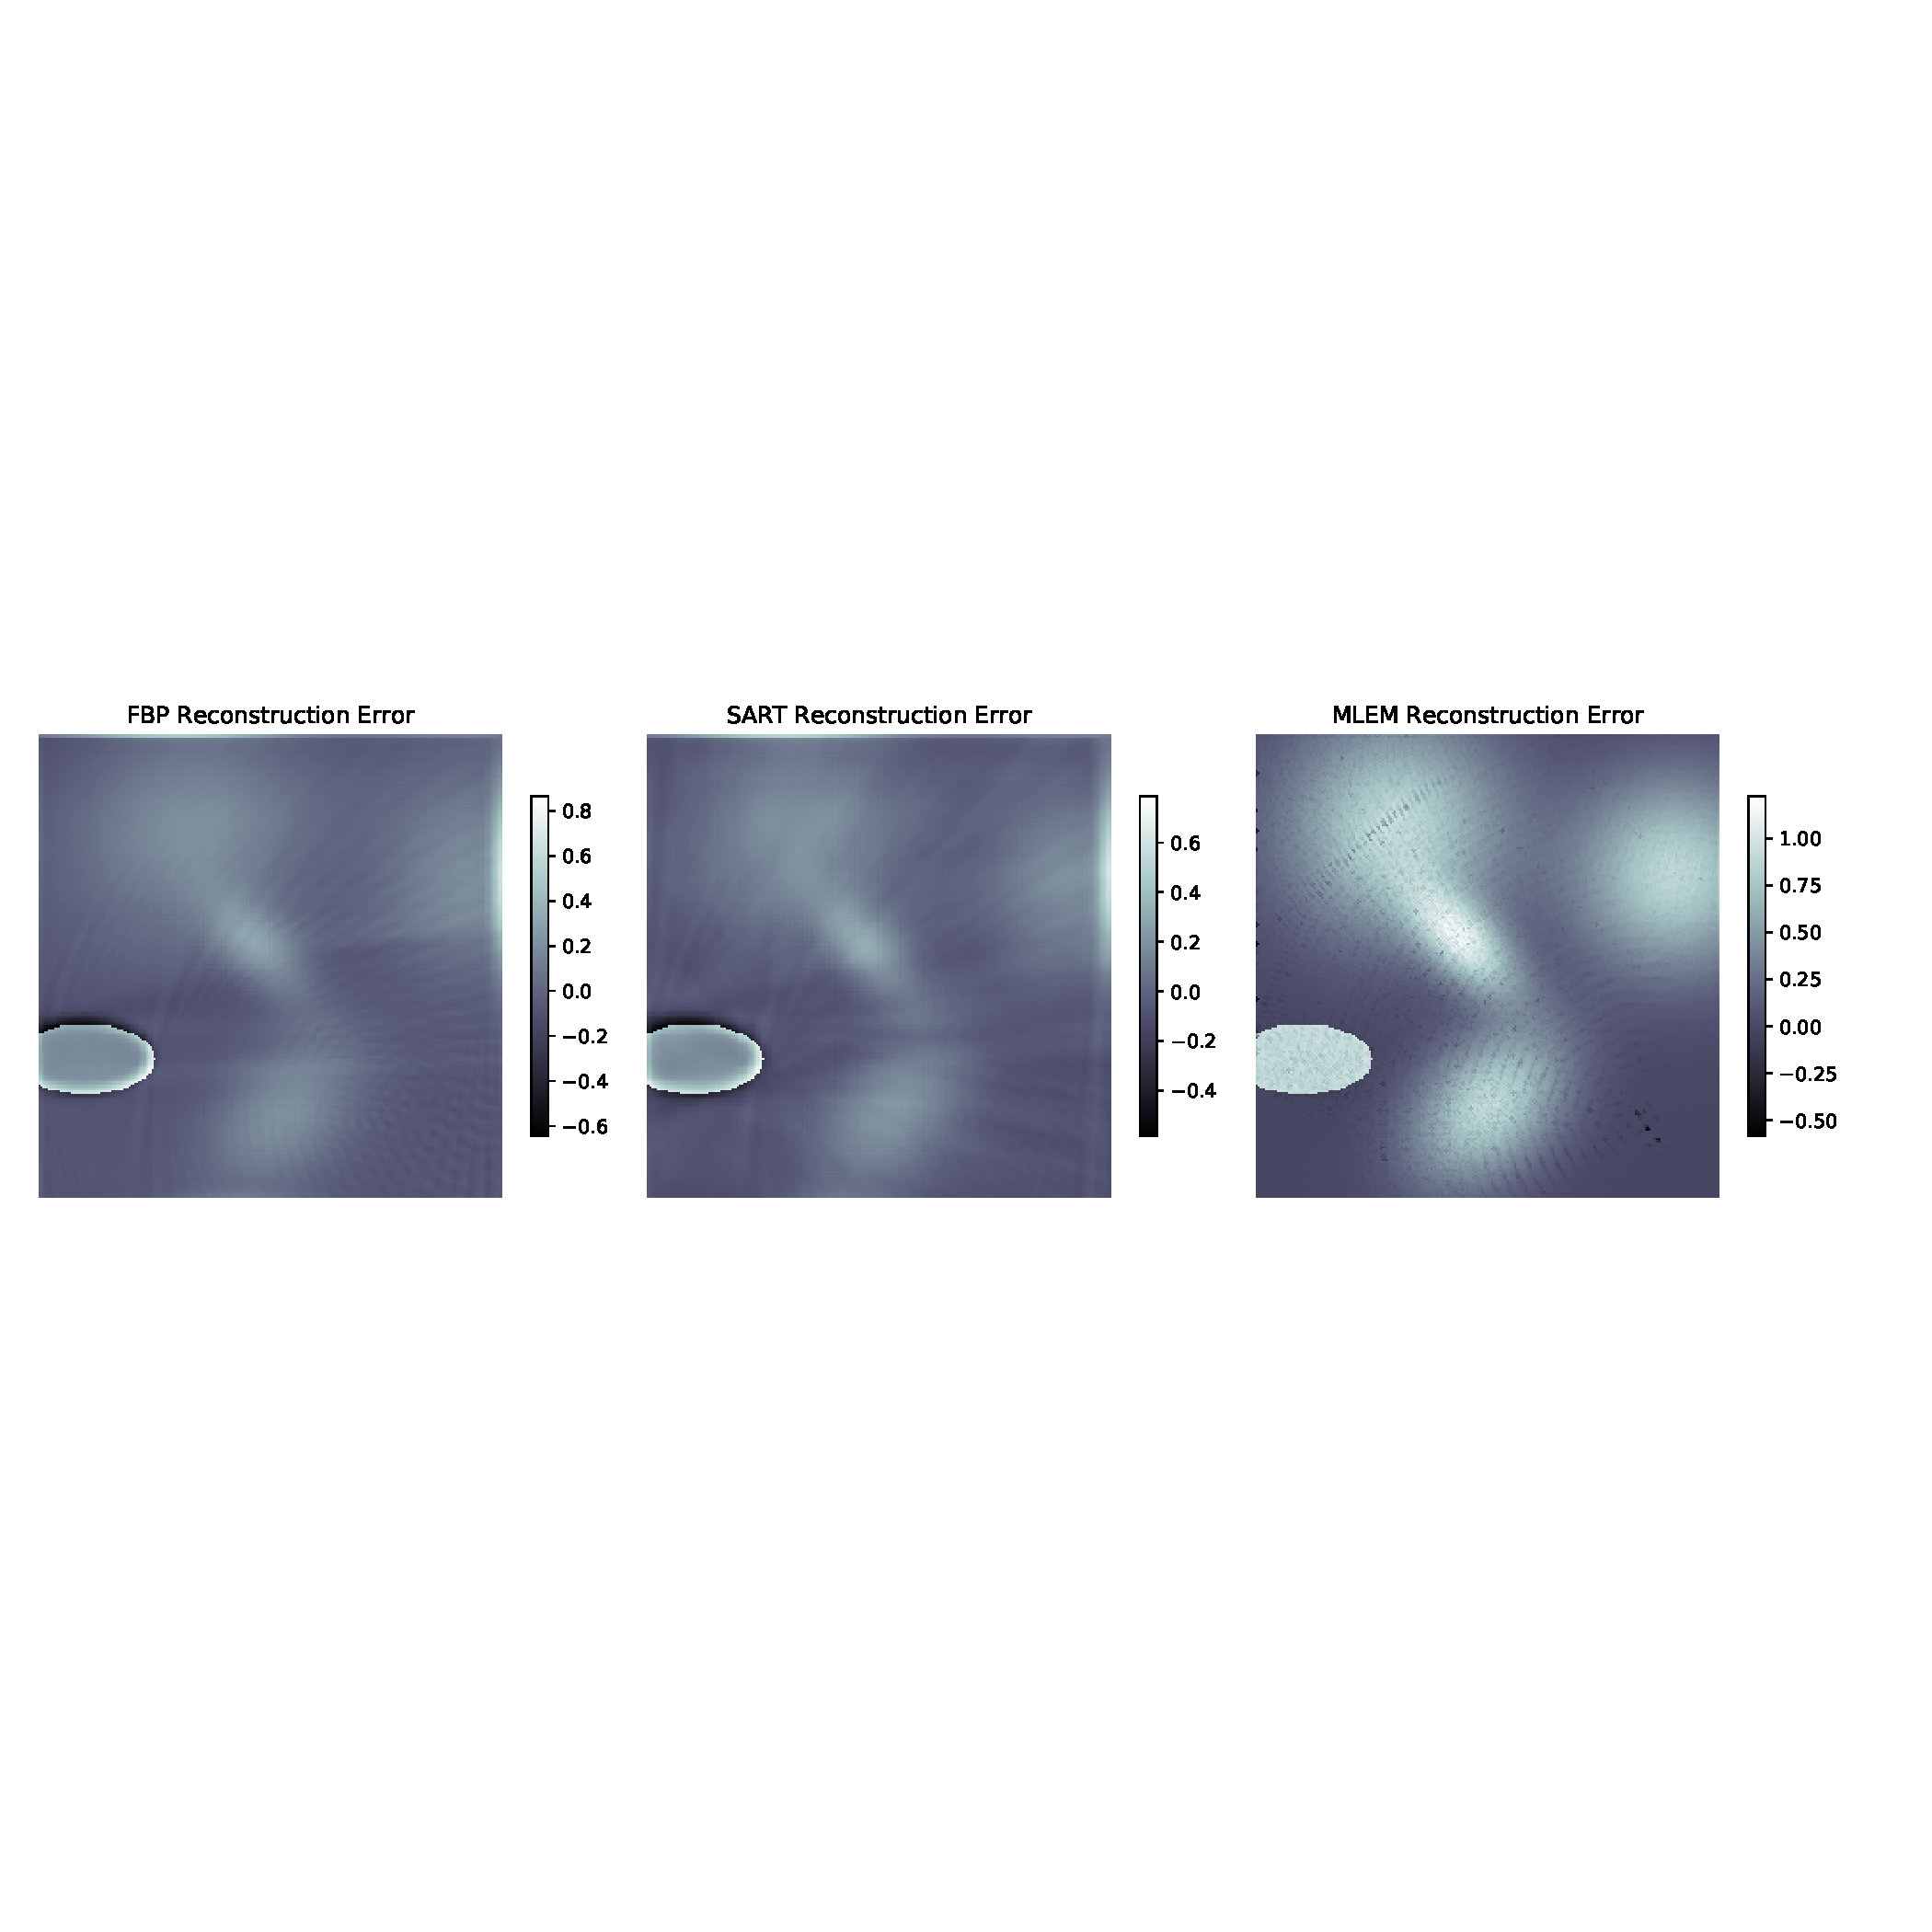
\includegraphics[clip, trim=.5cm 13.5cm 1.5cm 13cm,
    width=\textwidth]{img/pdf/rec_error_compilation_1.pdf}
    \caption{Tomographic reconstruction errors. Each one of these images
    was constructed by subtracting the respective reconstruction matrix,
    displayed in Figure~\ref{fig:rec_results}, from the original phantom
    matrix. Error value is normalised to the pixel values, i.e., 32 bit
    floating point numbers with values between 0 and 1.}
    \label{fig:rec_errors}
\end{figure*}

\begin{table}[h]
    \centering
    \caption{Reconstruction error table for the new spectral phantom at
    several projection intervals. The MLEM routine used pure fan-beam data
        while the other two used resorted parallel information. Errors
        presented were calculated using the Root Mean Square Errors,
        normalised to the range of the reconstructed image. }
    \label{tab:rec_errors}
    \begin{tabular}{lccccc}
    \toprule
    \multirow{2}{*}{\textbf{Algorithm}} & \multicolumn{5}{c}{\textbf{Projection Intervals}} \\ \cline{2-6} 
                                        & 1        & 2        & 3
                                        & 4       & 5       \\ \midrule
    \textbf{FBP}                        & 0,2365   & 0,2408   & 0,2609
                                        & 0,2948  & 0,3465  \\\midrule
    \textbf{SART}                       & 0,2225   & 0,2278   & 0,2771
                                        & 0,3537  & 0,3302  \\\midrule
    \textbf{MLEM}                       & 0,8705   & 0,9723   & 0,9986
                                        & 0,9744  & 0,9890  \\
                                        \bottomrule
    \end{tabular}
\end{table}

\begin{figure}[htpb]
    \centering
    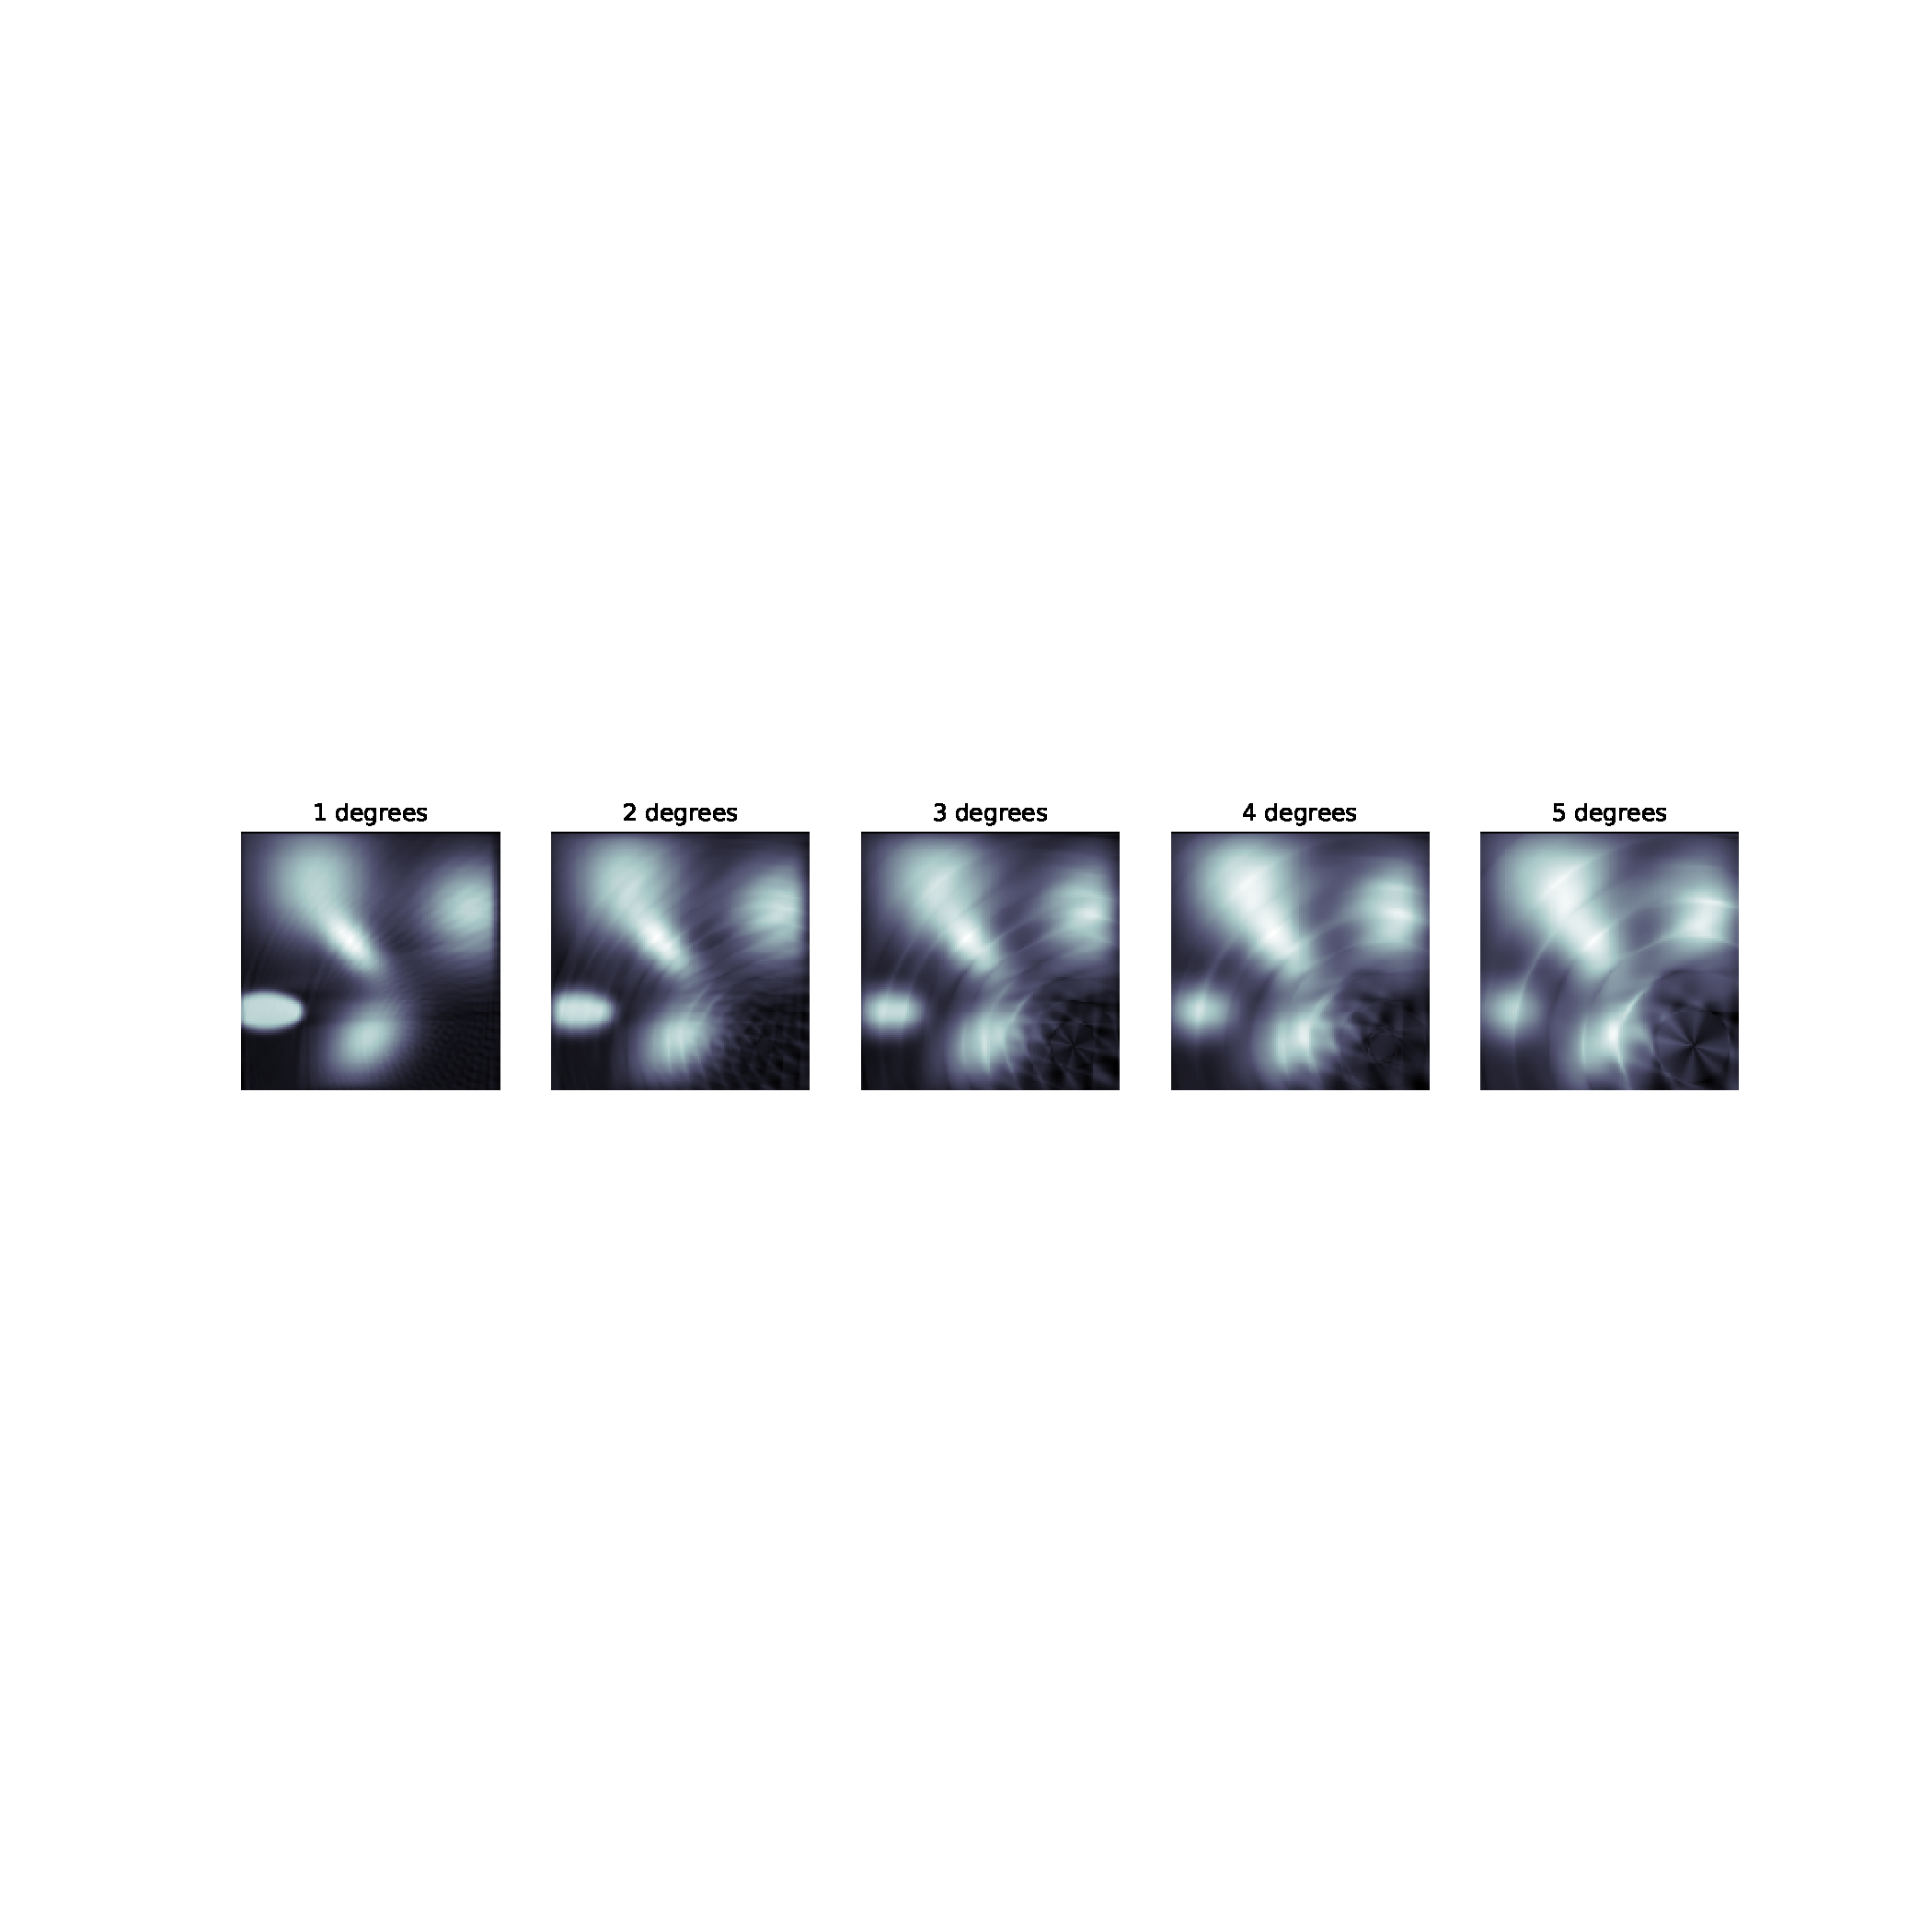
\includegraphics[clip, trim=4cm 15cm 3cm 14cm,
    width=\textwidth]{img/pdf/fbp_rec_degradation.pdf}
    \caption{Reconstruction degradation: the projection interval was
    crucial for reconstruction. Note the image degradation going from
    a projection interval of 1 degree to 5 degrees (left to right).
    Images reconstructed using the FBP algorithm.}
    \label{fig:rec_comparison}
\end{figure}
